\chapter{Introduction}
\label{intro}

In this chapter, diabetic retinopathy and diagnosis thereof is discussed. The chapter contains the potential benefits of automated detection of diabetic retinopathy and eye fundus images.  (Bu kisim degisecek - research question vs ekle)

\section{Diabetic Retinopathy}


\subsection{Structure of Eye}

\begin{figure}[t]
\centering
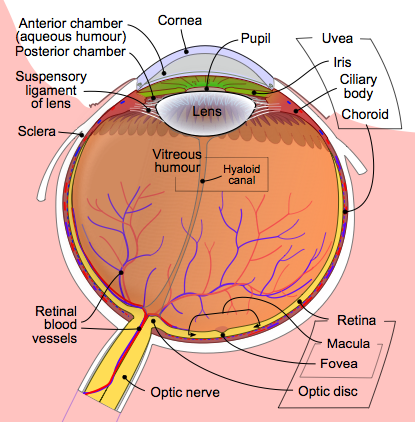
\includegraphics[width=0.8\textwidth]{Figures/structure_of_eye}
\caption{Structure of Human Eye \citep[from][]{WikipediaEN:AFM}}
\label{structureOfEye}
\end{figure}

As \citet{hughes2004anatomy} said, our sense organ of the eye, a ``window to the soul'', is of interest in many disciplines. (Buraya baglanti ekle) As seen on Figure~\ref{structureOfEye}, light reflected from an object enters the eye through the cornea, then passes through the pupil, and then the lens \citep{falt2012modern}, and is finally focused on retina. Depends on bright or dark, or distance of object eye regulates changes like amount of lights enters eye or focus on objects with pupil and reshaping elastic lens \citep{kauppi2010eye}. (Buraya baglanti ekle)

\begin{figure}[t]
\centering
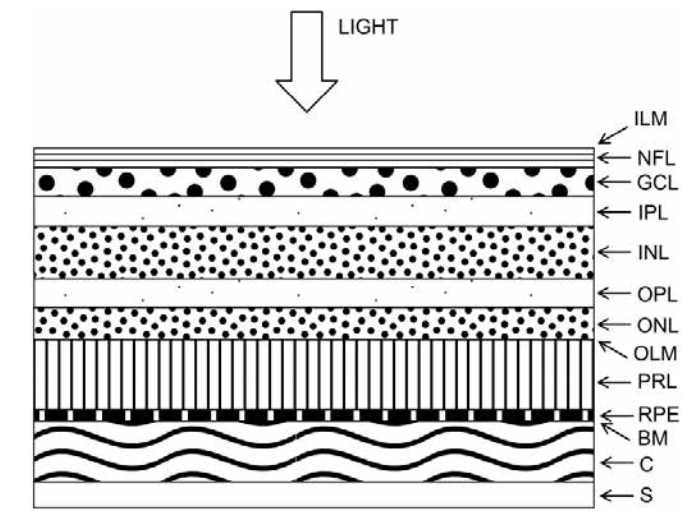
\includegraphics[width=0.8\textwidth]{Figures/layers_of_retina}
\caption{Cross-Section of Retina, Choroid (C), and Sclera (S) \citep[from][]{falt2012modern}}
\label{layersOfRetina}
\end{figure}


Before being transmitted to the rest of the brain for visual perception via the optic nerve, the information in the light is processed in layers of the retina \citep{kauppi2010eye}, which are shown in Figure~\ref{layersOfRetina}. The retina has 6 regions \citep{forrester2015eye}:
\begin{compactenum}
    \item Central retina
    \item Maculalutea
    \item Fovea centralis
    \item Optic disk
    \item Peripheral retina
    \item Ora serrata
\end{compactenum}
These anatomical parts of the retina are represented on one of the colour fundus images in the Messidor dataset \citep{mookiah2015application} described in Section~\ref{fundusPhotoRetina}. Their terminology is used in the remainder of this dissertation.

\begin{figure}[t]
\centering
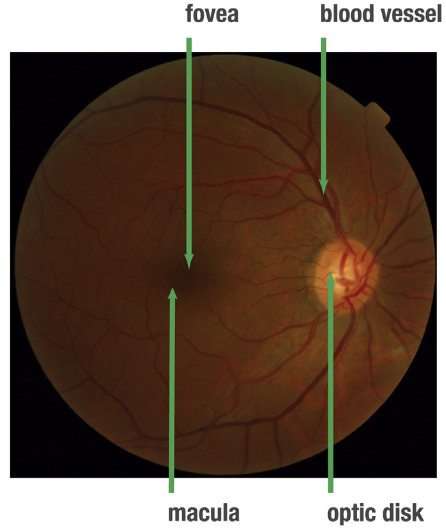
\includegraphics[width=0.8\textwidth]{Figures/fundus_photography_anatomical}
\caption{Fundus Image \citep[from][]{mookiah2015application}}
\label{fundusPhotoRetina}
\end{figure}


\subsection{Diabetes Mellitus and Diabetic Retinopathy}
The American Diabetes Association describes diabetes mellitus, which is a considered a global epidemic \citep{falt2012modern}, as a ``group of metabolic diseases characterised by hyperglycemia resulting from defects in insulin secretion, insulin action, or both'' \citep{national1979classification}. Diabetes mellitus can cause long term damage to the nervous system, kidneys, eye, etc. Diabetic retinopathy (DR) is the most common eye disease resulting from damage to the retina of the eye triggered by diabetes mellitus, and is a leading cause of vision loss in industrialised nations \citep{antal2014ensemble, stitt2013advances}. As a result of an increasing number of diabetes mellitus patients, worldwide blindness caused by diabetic retinopathy will become more common if treatment of diabetic retinopathy does not improve \citep{wilkinson2003proposed}. This is because diabetic retinopathy, if not cured during early stages of the disease, can cause the complete loss of sight \citep{rocha2011points}. 

In its early stages, patients do not have symptoms of diabetic retinopathy in their vision: the primary signs of early-stage DR are exudates \citep{nijalingappa2015machine}. In Figure~\ref{visionOfDrAndNodr}, there is a scene as seen by two different people; one with normal vision and and the other with black areas showing the visual percept of a person with advanced diabetic retinopathy \citep{NationalEyeInstitute}.

\begin{figure}[t]
\centering
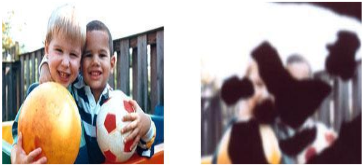
\includegraphics[width=0.8\textwidth]{Figures/vision_of_dr_and_nodr}
\caption{Scene viewed with normal vision (left) and advanced diabetic retinopathy (right).}
\label{visionOfDrAndNodr}
\end{figure}

Diabetic Retinopathy is divided into two main stages, depending on the precense of abnormal new blood vessels  \citep{tang2011inflammation, nijalingappa2015machine}: the nonproliferative stages (NPDR), which are the early stages of DR, and an advanced stage of DR, the proliferative stage (PDR).
During NPDR, DR progress in 3 stages:
    \begin{compactenum}
        \item Mild NPDR
        \item Moderate NPDR
        \item Severe NPDR
    \end{compactenum}


The \citet{NationalEyeInstitute} and \citet{wilkinson2003proposed} define these 4 stages of DR as follows:
\begin{enumerate}
        \item \textit{Mild NPDR:} This is the earliest stage of DR. In retinal capillaries, small changes starts. The smallest detectable abnormalities of DR, \textbf{microaneurysms (MA)}, are detectable as small red dots.
        \item \textit{Moderate NPDR:} The second stage of DR. Blood vessels may start to lose blood circulation ability and/or swell and distort. \textbf{Haemorrhages (HA)} starts to appear. These changes may cause diabetic \textbf{macular edema (DME)}.
        \item \textit{Severe NPDR:} Vessel blockage is increased in this stage; the retina starts to trigger the body's development of new vessels for supplying nutrition and oxygen to suffering areas. But these vessels are fragile and thin. \textbf{Intra-retinal microvascular abnormalities (IRMA)} are also signs of this stage. 
        \item \textit{PDR:} In the this stage, \textbf{neovascularisation}, which is the development of these new fragile vessels, starts. These fragile vessels  are dangeruous because they can cause sudden vision loss. \textbf{Soft exudates (cotton wool spots)} are visible in PDR. 
\end{enumerate}

Hard Exudates (HA), Haemorrhages (HA), and microaneurysms (MA) are shown in Figure~\ref{AbnormalitiesFundusImage}.

\begin{figure}[t]
\centering
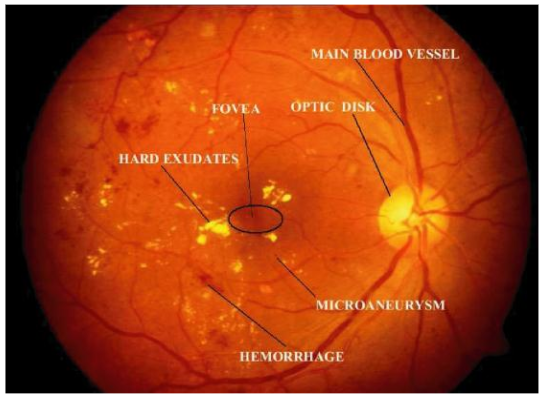
\includegraphics[width=0.8\textwidth]{Figures/retina_abnormalities}
\caption{Hard Exudate (HA), Haemorrhage (HA), and Microaneurysm (MA) Abnormalities on Fundus Image \citep[from][]{kekre2013hybrid}}
\label{AbnormalitiesFundusImage}
\end{figure}

\subsection{Diagnosing Diabetic Retinopathy}

This section explains how diabetic retinopathy is diagnosed, focusing on the main methods of diagnosis.

Early diagnosis of DR is very important to prevent vision loss in diabetes mellitus patients \citep{mankarautomatic}. Diagnosing DR is very difficult if diabetes mellitus is not suspected in the patient. DR is not visible in blood samples. These make DR a ``deceptive'' disease \citep{kauppi2010eye}. To detect DR, patient must take an extensive eye exam. \citet{kauppi2010eye} grouped these examinations as follows:
\begin{compactitem}
    \item Clinical eye examination,
    \item Eye fundus photography,
    \item Fluorescein angiography,
    \item Optical Coherence tomography (OCT).
\end{compactitem}
Since the 1980s, eye fundus photography has been available, and it has made opthalmoscopy the most commonly used examination method, if available, for diagnosis of DR \citep{wendt2005screening}. Eye fundus photography allows the data to be saved, allowing ophthalmologists to examine the image later \citep{hutchinson2000effectiveness}. 

\citet{rocha2011points} grouped diagnosis of anomalies of DR using the following titles, adding that diagnosing DR-non DR has recently become a popular approach for diagnosing DR:  
\begin{enumerate}
    \item \textbf{Detection of blood vessels:}  Because the eye is the only place where blood vessels can directly be observed in the human body, it is unique. DR causes changes to vascular conditions in the eye. Detection of any changes in the blood vessels is a way to diagnose DR from retinal fundus images \citet{mendonca2006segmentation}.
    \item \textbf{Detection of hard exudates:} Retinal oedema is the major cause of vision loss during the progress of DR. The existence of hard exudates indicates the presence of retinal oedema \citep{singer1992screening}, which is useful to ophthalmologists for both diagnosis and follow-up of DR \citep{garcia2009neural}.
    \item \textbf{Detection of microaneuysms:} In earliest stage of DR, microaneurysms and hemorrhages are visible \citep{doi:10.1056/NEJMra021678}. Hard exudates and cotton wool spots are not able to be detected in early stages of DR \citep{navarro2016automatic}. Because it is easier to prevent DR in earlier stages, detecting microaneuysms is important.
    \item \textbf{Detection of hemorrhages:} Hemorrhages are visible in early stages of DR, like microaneuysms, but this anomaly is more visible in advanced stages of DR: more hemorrhages means more retinal damage. In the literature, the following approaches are presented for detection of hemorrhages \citep{rocha2011points}:
    \begin{compactenum}
        \item Detection of blood vessels
        \item Detection of blood vessels with hemorrhages
    \end{compactenum}
\end{enumerate}

Algorithms and results used for these detections can be found in Chapter~\ref{related_work}.




\subsection{Screening Diabetic Retinopathy}

Can be extracted???? 


\section{Background (?)} 

\subsection{Restrictions}
\subsection{Contributions}



\section{Research Question(s)}
In this work we try to answer the following research questions:

\begin{itemize}
    \item Can signs of DR can be detected automatically by using machine learning algorithms, and in particular by using deep learning methods?
    \item Can we detect signs of DR in one dataset using a model trained on a different dataset?
    \item Will using deep learning on the task of DR detection open new research directions in this area? 
\end{itemize}

\section{Motivation}
According to National Eye Institute in the United States, in just the USA around 40--45\% of people with diabetes were diagnosed with diabetic retinopathy. Besides this, nearly 35\% of people with diabetes worldwide have DR, and 1 in 10 will have a vision-threatening form of the disease \citep{yau2012global}. According to recent work, diabetic retinopathy effects almost 4\% of the population of Europe \citep{nentwich2015diabetic}. Therefore, it is essential to detect the signs of DR in the early stages. The process of detecting the signs of diabetic retinopathy currently requires trained technicians to analyze the acquired diagnostic retinal images. Our main motivation is a desire to make this process automatic, using convolutional neural networks.

\section{Aims and Objectives}
As explained above, our main aim and goal is the automatic detection of the early signs of DR, using a wildly successful deep learning method, namely convolutional neural networks. We look for the results of using one large dataset for training, and other publicly available datasets for testing. 

\section{Reports Structure}
The structure of this document is as follows: in the next section we review the related work; then we explain our methodology, and describe the experimental setup and the result of the experiments. We end with a summary and a discussion of potential impact and possible future work.
